\documentclass[a4paper,12pt, twoside]{article}
%\documentclass[a4paper,12pt, twoside]{book}

\usepackage[papersize={210mm,297mm},tmargin=20mm,bmargin=20mm,lmargin=20mm,rmargin=20mm]{geometry}

\usepackage[utf8]{inputenc}
%https://mirror.hmc.edu/ctan/macros/latex/contrib/babel-contrib/turkish/turkish.pdf
\usepackage[english]{babel}
%\usepackage[T1]{fontenc}

\usepackage{amsmath,amssymb,mathabx}%\for eqref
\usepackage{lscape}

\usepackage{hyperref}
\hypersetup{
    colorlinks,
    citecolor=black,
    filecolor=black,
    linkcolor=blue,
    urlcolor=red}
  

%%% \usepackage{svg}
%%% https://tex.stackexchange.com/questions/122871/include-svg-images-with-the-svg-package/129854
\usepackage{graphicx}
\graphicspath{ {./figurler/} }

\usepackage[colorinlistoftodos]{todonotes}
\usepackage{fancyhdr}

\usepackage{indentfirst}
%% paragraf girintisi
\setlength{\parindent}{5ex}

%% Daha sonra yazılacak kısımları not düşmek için...
\newcommand{\YAZILACAK}{{\vspace{18pt}\bf\Large \color{red} YAZILACAK}}


\pagestyle{fancy}
\fancyhf{}
\lhead{ Kuantum Fiziği }
\chead{\thepage}
\rhead{Mesut Karakoç}
\lfoot{Akdeniz Üniversitesi}
\cfoot{}
%\rfoot{BF}

\title{Akdeniz Üniversitesi\\ Fen Fakültesi - Fizik Bölümü\\FİZ319 Kuantum Fiziği Ders Notları}

\author{\setlength{\unitlength}{6mm}
\begin{picture}(10,10)
\put(1.1,0){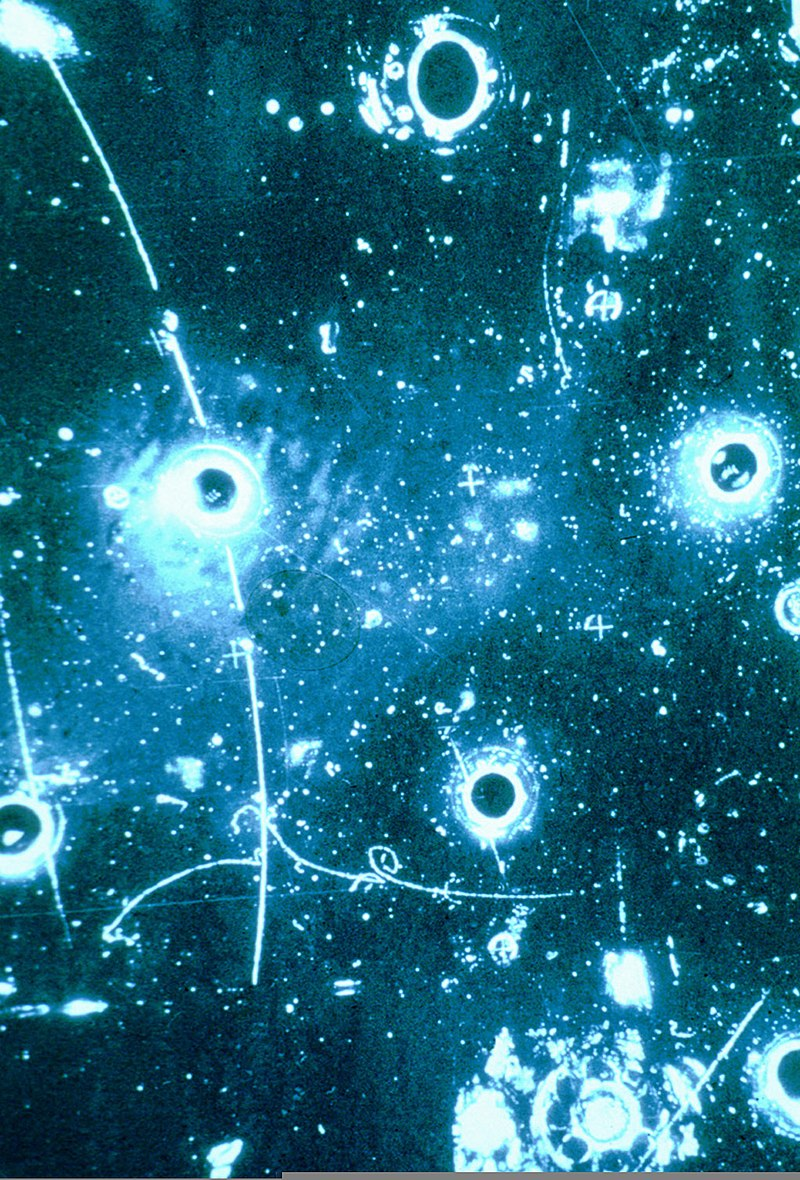
\includegraphics[width=4.5cm]{Leptonic_event_in_Gargamelle_bubble_chamber.jpg}}
\end{picture} \\ Doç. Dr. Mesut Karakoç}


\date{\today}

\begin{document}

%% Turkish babel problem
%% https://tex.stackexchange.com/questions/160385/newgeometry-doesnt-work-with-turkish-babel-package
%%\shorthandoff{=}% Make = not active any more

\maketitle

\newpage

% change name to "İçindekiler"
\renewcommand{\contentsname}{İçindekiler}
\tableofcontents{}

\listoffigures
 
\listoftables

\newpage

{
\hspace{.5\textwidth}
\begin{minipage}{.5\textwidth}
\raggedleft
If all this damned quantum jumps were really to stay, I should be
sorry I ever got involved with quantum theory.

—Erwin Schrödinger
\cite{book:Ficek}

%% Latince için
%% post iacturam quis non sapit!
%% Who is not wise after he has lost something?
%% https://quizlet.com/23756827/latin-proverbs-h-flash-cards/
\end{minipage}
}

\setcounter{section}{3} %% THIS WILL BE DELETED when all chapters merged!
\section{Bir Boyutlu Potansiyeller}

\YAZILACAK

\newpage
% In the preamble, add "\renewcommand\refname{New Title}" for article type documents 
% and "\renewcommand\bibname{New Title}" for book and report type documents.
\renewcommand\refname{Kaynaklar}
\bibliography{quantumBIB}{}
%% https://www.sharelatex.com/learn/latex/bibtex_bibliography_styles
 \bibliographystyle{plain}
%% \bibliographystyle{alpha}
%%\bibliographystyle{apalike}
\end{document}

